\documentclass[twoside]{article}
\usepackage{aistats2014}
\usepackage{amsthm,amsmath}
\usepackage{amssymb}
\usepackage[boxed]{algorithm2e}
\usepackage{bm}
\usepackage{bbm}
\usepackage{url}
\usepackage{comment}
\usepackage{url}
\usepackage{multirow}
\usepackage{graphicx}
\usepackage{color}
\usepackage{tikz}

% If your paper is accepted, change the options for the package
% aistats2014 as follows:
%
%\usepackage[accepted]{aistats2014}
%
% This option will print headings for the title of your paper and
% headings for the authors names, plus a copyright note at the end of
% the first column of the first page.


\begin{document}

% If your paper is accepted and the title of your paper is very long,
% the style will print as headings an error message. Use the following
% command to supply a shorter title of your paper so that it can be
% used as headings.
%
%\runningtitle{I use this title instead because the last one was very long}

% If your paper is accepted and the number of authors is large, the
% style will print as headings an error message. Use the following
% command to supply a shorter version of the authors names so that
% they can be used as headings (for example, use only the surnames)
%
%\runningauthor{Surname 1, Surname 2, Surname 3, ...., Surname n}

\newtheorem{definition}{Definition}[section]
\newtheorem{theorem}{Theorem}[section]
\newtheorem{lemma}{Lemma}[section]
\newtheorem{corollary}{Corollary}[section]

\def\layersep{2cm}
\def\layersepp{4cm}

\twocolumn[

\aistatstitle{Complexity of large neural networks}

\aistatsauthor{ Anonymous Author 1 \And Anonymous Author 2 \And Anonymous Author 3 }
%\aistatsauthor{
%\And
%Anna Choromanska \\
%\texttt{achoroma@cims.nyu.edu} \\
%\And
%Mikael Henaff\\
%\texttt{mbh305@nyu.edu} \\
%\And
%Michael Mathieu\\
%\texttt{mathieu@cs.nyu.edu}\\
%\And
%Levent Sagun\\
%\texttt{sagun@cims.nyu.edu} \\
%\And
%Yann LeCun\\
%\texttt{yann@cs.nyu.edu} \\
%}

\aistatsaddress{ Unknown Institution 1 \And Unknown Institution 2 \And Unknown Institution 3 } ]
%\aistatsaddress{
%Courant Institute of Mathematical Sciences \\
%New York University\\
%New York, NY 10012 \\
%}]

\begin{abstract}
We explore the approximate relation between the highly non-convex loss function of a simple model of the fully-connected feed-forward neural network and the Hamiltonian of the spherical spin-glass model under certain assumptions. Using the results from the random matrix theory, we study the complexity of neural networks and prove that for large-size networks the lowest critical values of the loss function are located in a well-defined narrow band lower-bounded by the global minimum and furthermore they form a layered structure. Moreover, finding them outside the band diminishes exponentially with the size of the network. We empirically demonstrate that both simulated annealing and SGD converges to the band of the lowest critical values, and furthermore all critical points found there are local minima and correspond to the same high learning quality measured by the test error. This emphasizes a major difference between large- and small-size networks where for the latter poor quality local minima have non-zero probability of being recovered. Simultaneously we prove that recovering the global minimum diminishes with the network size and that it is in practice irrelevant as global minimum often leads to data overfitting. 
\end{abstract}

\section{Introduction}

Neural networks are machine learning models used for learning complex and highly non-linear mathematical functions in the context of regression, classification, pattern recognition, clustering, reinforcement learning etc. Modern neural networks historically originate from simple early models such as threshold logic~\cite{mcculloch43a}, Hebbian network~\cite{Hebb:1949} and perceptron~\cite{rosenblatt58a} that were followed by more sophisticated models including Hopfield network~\cite{Hopfield:1988:NNP:65669.104422}, Kohonen network~\cite{Kohonen1982}, and Boltzman machines~\cite{Hinton:1986:LRB:104279.104291} (and many others). Despite their modeling power, the interest in learning with early neural network significantly weakened when it was shown that they have several limitations including: i) learning limitations such as the inability of single-layer networks to solve the XOR problem~\cite{minsky69perceptrons}, ii) long training time of large networks and proness to overfitting~\cite{JMLR:v15:srivastava14a}, and iii) getting stuck in poor-quality local optima or saddle points while training~\cite{Larochelle:2009:EST:1577069.1577070}. Today many of these limitations can be solved with the development of new efficient training strategies (among them backpropagation algorithm~\cite{Werbos:74} which enables to solve the XOR problem), fast GPU-based implementations significantly reducing the training time, and techniques preventing the overfitting such as dropout (e.g.~\cite{JMLR:v15:srivastava14a}). Therefore, after a long period of scepticism, the paradigm of learning with neural networks gained significant attention in recent years resulting in many new architectures, such as convolutional networks~\cite{lecun-gradientbased-learning-applied-1998}, recurrent neural networks~\cite{Graves:2009:NCS:1525650.1525782}, deep feedforward neural networks (e.g.~\cite{DBLP:journals/corr/Schmidhuber14} or wide networks~\cite{Huang14}, where the most fundamental difference between them and their early predecessors lies in a much larger parameter space (throughout the paper we refer to the number of network parameters as network size). In effect, the optimization problem arising when training these models is highly non-convex with exponentially many critical points. Despite the apparent difficulty of this optimization, modern neural network approaches often beat state-of-the-art results on a plethora of learning tasks (pattern recognition~\cite{journals/nn/CiresanMMS12}, brain image segmentation~\cite{NIPS2012_4741}, human pose estimation~\cite{DBLP:journals/corr/TompsonJLB14}, large-scale visual recognition~\cite{sermanet-iclr-14}, transfer learning~\cite{conf/icml/GoodfellowCB12} and many more) which is highly suggestive of their ability to recover high-quality solution to the optimization problem. The fundamental question arises: 'Why?' 

The paradigm of optimizing a highly non-convex loss function characteristic of modern neural newtorks remains largely ununderstood with a lot of empirical evidence and almost no theoretical justification (the overview of prior work is done in Section~\ref{sec:PriorWork}). That results in often perceiving these models as 'black box' tools and rejecting them in favor of significantly simpler models which training is based on solving convex optimization problem. Convex optimization problems due to having no local optima are well-understood and nearly-exactly (or exactly) solvable by many standard efficient optimizers with known theoretical convergence guarantees in this setting (some standard results can be found in~\cite{opac-b1104789, ben-tal_nemirovski:2001}). The goal of this paper is to provide insights to the paradigm of large-size neural network optimization where the problem is highly non-convex. We establish the connection between the loss function (we focus on hinge loss and absolute loss) of the fully-connected one-output feed-forward neural network of depth $H$ with the Hamiltonian of the $H$-spin spherical spin-glass model. We show that the latter can be thought of us an approximator of the loss function of the network under certain assumptions which we also discuss, and furthermore we provide the theoretical guarantee of the quality of this approximation. Through the prism of recent findings in random matrix theory~\cite{AAC2010}, in Section~\ref{sec:theory} we study the complexity, i.e. the exponential behavior of the mean number of critical points (in total and of given index), of neural networks. We prove that for large-size networks the local minima and low-index saddle points of the loss function lie within a narrow band lower-bounded by the global minimum and finding them outside the band diminishes exponentially with the size of the network. Furthermore, within the band, the lowest critical points form a very well-defined layered structure that we also describe in the paper. Finally, recovering the global minimum of the loss function diminishes with network size. In the experimental section (Section~\ref{sec:Experiments}) we empirically verify several hypotheses regarding learning with large-size networks:
\vspace{-0.05in}
\begin{itemize}
\item For large-size networks local minima are equivalent and correspond to the same quality solution measured by the test error.
\vspace{-0.05in}
\item Probability of finding a poor quality local minima is non-zero for small-size networks and it exponentially diminishes with the network size.
\vspace{-0.05in}
\item Finding the global minimum on the training set is not useful in practice as it often leads to overfitting.
\vspace{-0.05in}
\item The local minima are mostly flat and are characterised by Hessian with mostly zero eigenvalues. This is an indication that large-size networks can be simplified.
\vspace{-0.05in}
\item The number of positive eigenvalues of the Hessian at local minima is invariant to network size.
\end{itemize}
\vspace{-0.05in}
The first three hypotheses can be directly justified by our theoretical findings and the last two are provided as corollaries without proof but with strong empirical evidence. We finally conclude the paper with brief discussion of our results and future research directions in Section~\ref{sec:ConandFutWork}. 

What is new in this paper? To the best of our knowledge, this paper is the first work providing a theoretical description of the optimization paradigm with neural networks in the presence of large number of parameters. It is also an attempt to make the modern neural network approach more a provable machine learning method and move it away from the 'black-box' shadow. We provide new insights explaining why this approach achieve high practical performance supported by the theoretical analysis and empirical verification.

\section{Prior work}
\label{sec:PriorWork}

Machine learning problems are most often formulated as optimization problems, majority of which are convex. It is often the case however that introducing non-convextiy into the model results in better practical performance~\cite{Do:2012:RBM:2503308.2503355, Bengio+chapter2007}. A typical examples of models giving rise to non-convex problems are neural networks, mixture models, models exploring products of parameters or those with complex non-linearities imposed on parameters. Better expressiveness of those models come with a price: the landscape of their objective functions is not-well understood as it contains several local optima. Thus those models typically are provided with no theoretical description. 

To the best of our knowledge the recent work of~\cite{DBLP:journals/corr/DauphinPGCGB14} is the first one to explore the statistical properties of neural network error surfaces through the prism of statistical physics and random matrix theory. In particular these theoretical works~\cite{Bray2007,Fyodorov2007,Baldi:1989:NNP:70359.70362,wigner_semicircle} suggest the existence of a certain structure of critical points of random Gaussian error functions on high dimensional continuous spaces. They imply that critical points which error is much higher than the global minimum are exponentially likely to be saddle points with many negative and approximate plateau directions whereas all local minima are likely to have an error very close to that of the global minimum (these results are conveniently reviewed in~\cite{DBLP:journals/corr/DauphinPGCGB14}). The work of~\cite{DBLP:journals/corr/DauphinPGCGB14} establishes a strong connection between neural networks and the theory of random Gaussian fields through an empirical evaluation by providing an experimental evidence that the cost function of neural networks exhibits the same properties as the Gaussian error functions on high dimensional continuous spaces. Nevertheless they provide no theortical justification for the existence of this connection which instead we provide in this paper. \textcolor{red}{We should comment why saddle-point problem in not a problem for us.}

This work is inspired by the recent advances in random matrix theory and the work of~\cite{AAC2010} and~\cite{AAC2013}. The authors of these works provided an asymptotic evaluation of the complexity of the spherical spin-glass model (the spin-glass model originates from the condensed matter physics where it is used to represent a magnet with irregularily aligned spins). They discovered and mathematically proved the existence of a layered structure of the low critical values for the model's Hamiltonian which in fact is a Gaussian process. Their results are not discussed in details here as it will be done in Section~\ref{sec:theory} in the context of neural networks. We build the bridge between their findings and neural networks and show that the objective function used by neural network is analogous to the Hamiltonian of the spin-glass model and thus their landscapes share the same properties. We emphasize that the connection between spin-glass models and neural networks was already explored back in the past (a summary can be found in~\cite{Dotsenko1995}). In example in~\cite{PhysRevA.32.1007} the authors showed that the long-term behavior of certain neural network models are governed by the statistical mechanism of infinite-range Ising spin-glass Hamiltonians. Another work~\cite{0305-4470-30-23-009} examined the nature of the spin-glass transition in the Hopfield neural network model. None of these works however make the attempt to explain the paradigm of optimizing the highly non-convex neural network objective function through the prism of spin-glass theory and thus in this respect our approach is very novel.

\section{Deep network and spin-glass model}
\label{sec:NNSG}

\subsection{Preliminaries}

For the theoretical analysis, we consider a simple model of the fully-connected feed-forward deep network with a single output and rectified linear units. We call the network $\mathcal{N}$. We focus on a binary classification task. Let $X$ be the random input vector of dimensionality $d$. Let $(H-1)$ denote the number of hidden layers in the network and we will refer to the input layer as the $0^{\text{th}}$ layer and to the output layer as the $H^{\text{th}}$ layer. Let $n_i$ denote the number of units in the $i^{\text{th}}$ layer (note that $n_0 = d$ and $n_H = 1$). Let $W_i$ be the matrix of weights between $(i - 1)^{\text{th}}$ and $i^{th}$ layers of the network. Also, let $\sigma$ denotes the activation function that converts a unit's weighted input to its output activation. We consider linear rectifiers thus $\sigma(x) = \max(0,x)$. We can therefore write that for any given random input vector $X$, the network gives the following (random) output $Y$:
\[Y = q\sigma(W_H^{\top}\sigma(W_{H-1}^{\top}\dots\sigma(W_1^{\top}X)))\dots),
\]
where $q = \sqrt{\frac{n_0n_1 + n_1n_2 + ... + n_{H-1}n_H}{n_0n_1...n_H}}$ is simply a normalization factor. The same expression for the output of the network can be re-expressed in the following way:
\begin{equation}
Y = q\sum_{i=1}^{n_0}\sum_{j = 1}^\gamma X_{i}A_{i,j}\prod_{k = 1}^{H}w_{i,j}^{(k)},
\label{eq:befrein}
\end{equation}
where the first summation is over the network inputs and the second one is over all paths from a given network input to its output, where $\gamma$ is the total number of such paths (note that $\gamma = n_1n_2\dots n_H$). Furthermore, $w_{i,j}^{(k)}$ is the weight of the $k^{\text{th}}$ segment of path indexed with $(i,j)$ which connects layer $(k-1)^{st}$ with layer $k^{\text{th}}$ of the network. Note that each path corresponds to a certain set of $H$ weights, which we refer to as a \textit{configuration of weights}, which are multiplied by each other. Finally, $A_{i,j}$ denotes whether a path $(i,j)$ is active ($A_{i,j} = 1$) or not ($A_{i,j} = 0$). 

\begin{definition}
The mass of the network $\Psi$ is the total number of all paths between all network inputs and outputs: $\Psi = \prod_{i=0}^Hn_i$.
\end{definition}

\begin{definition}
The size of the network $\Lambda$ is the total number of network parameters: $\Lambda = \sum_{i=0}^{H-1}n_in_{i+1}$.
\end{definition}

There mass and the size of the network depend on each other as captured in Theorem~\ref{thm:arge}.
\begin{theorem}
Let $\Psi$ be the mass of the network, $d$ be the number of network inputs and $H$ be the depth of the network. The size of the network is bounded as
\[\Psi^2\frac{1}{d} \geq \Lambda \geq \sqrt[H]{\Psi^2}\frac{H}{\sqrt[H]{d}} \geq \sqrt[H]{\Psi}.
\]
\label{thm:arge}
\end{theorem}

In the rest of this section we will be establishing a connection between the loss function of the neural network and the Hamiltonian of the spin-glass model. Under certain assumptions, that will be introduced and discussed, spin-glass model can be though of as an approximator of a network output. We will also provide the measure of quality of this approximation. All proofs are deferred to the Supplementary material.

\subsection{Approximation}

In this section we introduce randomness to the model and assume $X$s and $A$s are random. We make certain assumptions regarding the neural network model. These assumptions consider random variables $X$s and $A$s (their distributions and mutual dependencies and we emphasize that all independence assumptions we make are standard in the literature~\cite{opac-b1095246}) as well as they introduce spherical constraint on the model weights. We also introduce two other assumptions regarding redundancy of network parameters and their uniformity (details in the text below), both of them are justified by empirical evidence in the literature. The aim of this section is to obtain an approximator to the expectation $\mathbb{E}_A[Y]$ (note it is still a random variable) which, as will be seen in Section~\ref{subsec:LFSG}, is used in the definition of the loss function of neural network. Theorems~\ref{thm:redun} and~\ref{thm:unif} provide some guarantees regarding the quality of this approximation.  

\paragraph{Input}
We assume each input $X_i$ is a normal random variable such that $X_i\sim N(0,1)$. 

\paragraph{Equally likely paths}
We assume each path in Equation~\ref{eq:befrein} is equally likely to be active thus $A_{i,j}$'s will be modelled as Bernoulli random variables with the same probability of success $\rho$. By assuming the independence of $X$'s and $A's$ we get the following
\begin{equation}
\mathbb{E}_A[Y] = q\sum_{i=1}^{n_0}\sum_{j = 1}^\gamma X_{i}\rho\prod_{k = 1}^{H}w_{i,j}^{(k)}.
\label{eq:befrein2}
\end{equation}

\paragraph{Spherical constraint}
Let $\mathcal{W} = \{w_1,w_2,\dots,w_{\Lambda}\}$ be the set of all weights of the network. We make a benign assumption that the weights sattisfy the spherical condition 
\begin{equation}
\frac{1}{\Lambda}\sum_{i=1}^{\Lambda}w_i^2 = \mathcal{C},
\label{eq:befspherical}
\end{equation}
where $\mathcal{C}$ is some positive constant. 

\paragraph{Redundancy in network parametrization}
Let $\mathcal{A}$ denote the set of all $H$-length configuration of weights chosen from $\mathcal{W}$ (order of weights in a configuration does matter). Note that the size of $\mathcal{A}$ is therefore $\Lambda^H$. Also let $\mathcal{B}$ be a set such that each element correspond to the single configuration of weights from Equation~\ref{eq:befrein2}, thus $\mathcal{B} = \{(w_{1,1}^1,w_{1,1}^2,\dots,w_{1,1}^H),(w_{1,2}^1,w_{1,2}^2,\dots,w_{1,2}^H),\dots,\\(w_{n_0,\gamma}^1,w_{n_0,\gamma}^2,\dots,w_{n_0,\gamma}^H)\}$, where every single weight comes from set $\mathcal{W}$. Note that in general there exist elements in $\mathcal{A}$ that will never appear in $\mathcal{B}$ (unless we allow repetition of weights in $\mathcal{W}$). Thus Equation~\ref{eq:befrein2} can be equivalently written as 
\begin{equation}
Y_{\Lambda} \!:=\! \mathbb{E}_A[Y] \!=\! q\!\!\!\!\sum_{i_1,i_2,\dots,i_H=1}^{\Lambda}\!\!\!\!\!\!\!\!\!\!\!r_{i_1\!,i_2,\dots,i_H}\!X_{i_1,i_2,\dots,i_H}\rho\!\prod_{k = 1}^{H}\!\!w_{i_k},
\label{eq:befapprox}
\end{equation}
where $r_{i_1,i_2,\dots,i_H}$ denotes whether the configuration $(w_{i_1},w_{i_2},\dots,w_{i_H})$ appeared in Equation~\ref{eq:befrein2} or not thus $r_{i_1,i_2,\dots,i_H} \in \{0\cup{1}\}$ and furthermore $\sum_{i_1,i_2,\dots,i_H=1}^{\Lambda}r_{i_1,i_2,\dots,i_H} = \Psi$. In the notation $Y_{\Lambda}$, index $\Lambda$ refers to the number of unique weights of a network (this notation will be helpful later in this section).  

Consider a family of networks which have the same graph of connections as network $\mathcal{N}$ but different edge weighting such that they only have $s$ unique weights and $s \leq \Lambda$ (through notation analogy expected output of this network will be called $Y_s$). It was recently shown~\cite{NIPS2013_5025,DBLP:journals/corr/DentonZBLF14} that for large-size networks large number of network parameters (according to~\cite{NIPS2013_5025} even up to $95\%$) are reduntant and can either be learned from a very small set of unique parameters or even not learned at all with almost no loss in prediction accuracy.  In our experimental section we also demonstrate the empirical evidence of the overparametrization of neural networks. It is therefore well-justified to \textit{assume redunancy in network parametrization} where $s$ is the number of unique (non-redundant) parameters.

\begin{definition}
A network $\mathcal{M}$ which has the same graph of connections as $\mathcal{N}$ and the number of unique weights $s$ satisfying $s \leq \Lambda$ is called a $(s,\epsilon)$-\textit{reduction image} of $\mathcal{N}$ for some $\epsilon \in [0,1]$ if the prediction accuracy of $\mathcal{N}$ and $\mathcal{M}$ differ by no more than $\epsilon$ (thus they classify at most $\epsilon$ fraction of data points differently).
\end{definition}

\begin{theorem}
Let $\mathcal{N}$ be a neural network giving the output whose expectation $Y_{\Lambda}$ is given in Equation~\ref{eq:befapprox}. Let $\mathcal{M}$ be its $(s,\epsilon)$-reduction image for some $s \leq \Lambda$ and $\epsilon \in [0,p]$. Through analogy, let $Y_s$ be the expected output of network $\mathcal{M}$. Then the following holds
\[corr(sign(Y_s),sign(Y_{\Lambda})) \geq \frac{1-2\epsilon}{1+2\epsilon},
\]
where $corr$ denotes the correlation defined as $corr(A,B) = \frac{\mathbb{E}[(A - \mathbb{E}[A]])(B - \mathbb{E}[B]])}{std(A)std(B)}$, $std$ is the standard deviation and $sign(\cdot)$ denotes the sign of prediction ($sign(Y_s)$ and $sign(Y_{\Lambda})$ are both random).
\label{thm:redun}
\end{theorem}

The assumption of the redundancy of parameters implies that one can preserve $\epsilon$ to be close to $0$ even with $s << \Lambda$.

\paragraph{Uniformity}
Consider $(s,\epsilon)$-reduction image of $\mathcal{N}$ for some $s \leq \Lambda$ and $\epsilon \in [0,1]$. The output $Y_s$ of the image network can in general be expressed as
\[Y_s = q\!\!\!\sum_{i_1,\dots,i_H=1}^{s}\!\!\!\sum_{j=1}^{r_{i_1,\dots,i_H}^{'}}X_{i_1,\dots,i_H}^{(j)}\rho\prod_{k = 1}^{H}\!\!w_{i_k},
\]
where $r_{i_1,\dots,i_H}^{'} \in \{\mathbb{Z}^{+}\cup{0}\}$ is the number of times each configuration $(w_{i_1},w_{i_2},\dots,w_{i_H})$ repeats in Equation~\ref{eq:befapprox} and $\sum_{i_1,\dots,i_H=1}^{s}r_{i_1,\dots,i_H}^{'} = \Psi$. We can further rewrite $Y_s$ as follows
\[Y_s = q\!\!\!\sum_{i_1,\dots,i_H=1}^{s}\!\!\underbrace{\left(\!\sum_{j=1}^{r_{i_1,\dots,i_H}^{'}}\!\!\!X_{i_1,\dots,i_H}^{(j)} + 0 + \dots + 0\right)}_{r_{i_1,\dots,i_H}^{''} \text{summands}}\!\!\rho\prod_{k = 1}^{H}\!\!w_{i_k},
\]
where $r_{i_1,\dots,i_H}^{''} \in \{\mathbb{Z}^{+}\cup{0}\}$ is the number of times each configuration $(w_{i_1},w_{i_2},\dots,w_{i_H})$ would repeat in Equation~\ref{eq:befapprox} if all $r_{i_1,\dots,i_H}$ would be equal to $1$ and $\mathcal{W}$ would have $s$ unique weights and the remaining $(\Lambda - s)$ weights were repetitions\footnote{Note that each $r_{i_1,\dots,i_H}^{''}$ is not uniquely defined here as one could consider many different ways of constructing $\mathcal{W}$ by repeating the same weights different times.}. We therefore require that $r_{i_1,\dots,i_H}^{''} \in \{\mathbb{Z}^{+}\cup{0}\}$, $r_{i_1,\dots,i_H}^{''} \geq r_{i_1,\dots,i_H}^{'}$ and $\sum_{i_1,\dots,i_H=1}^{s}r_{i_1,\dots,i_H}^{''} = \Lambda^H$. Let $\hat{r}_{i_1,\dots,i_H} = \sqrt{\frac{r_{i_1,\dots,i_H}^{'}}{r_{i_1,\dots,i_H}^{''}}}$ and for convinience assume that $\frac{1}{\hat{r}_{i_1,\dots,i_H}^2} \in \mathbb{Z}^{+}$. By the infinite divisibility property of normal distribution we can decompose each $X_{i_1,\dots,i_H}^{(j)}$ as the sum of $\frac{1}{\hat{r}_{i_1,\dots,i_H}^2}$ independent normal random variables (we call them $Z$'s). Thus
\[X_{i_1,\dots,i_H}^{(j)} = \hat{r}_{i_1,\dots,i_H}\sum_{k=1}^{\frac{1}{\hat{r}_{i_1,\dots,i_H}^2}}Z_{i_1,\dots,i_H}^{(j,k)}.
\]
Furthemore, this decomposition is not unique. This enables us to prove (proof is in the Supplementary material) the following result that we give as a lemma.
\begin{lemma}
The decomposability of the input $X_{i_1,\dots,i_H}^{(j)}$ implies that
\[Y_s = q\sum_{i_1,\dots,i_H=1}^{\Lambda}\hat{r}_{i_1,\dots,i_H}Z_{i_1,\dots,i_H}\rho\prod_{k = 1}^{H}w_{i_k},
\]
where $Z$'s are independend standard normal random variables.
\label{lem:tmp2}
\end{lemma}

Finally we assume that unique weights are close to being evenly distributed on the graph of connections of network $\mathcal{M}$. We call this assumption a \textit{uniformity assumption} (note it is analogous to the maximum entropy assumption). This assumption is in general consistent with the approach in~\cite{NIPS2013_5025}. To be more specific, this assumption implies that for all $(i_1,i_2,\dots,i_H):i_1,i_2,\dots,i_H \in \{1,2,\dots,H\}$ there exists non-negative constant $c$ and $\delta \in [0,1]$ such that the following holds
\begin{equation}
c\delta\sqrt{\frac{\Psi}{\Lambda^H}} \leq \hat{r}_{i_1,i_2,\dots,i_H} \leq c\sqrt{\frac{\Psi}{\Lambda^H}},
\label{eq:uniform}
\end{equation}
where the factor $\sqrt{\frac{\Psi}{\Lambda^H}}$ comes from the fact that for the network where every weight is uniformly distributed on the graph of connections (thus every node has equal probability of being adjacent to an edge with any of the unique weights) it holds that $\hat{r}_{i_1,i_2,\dots,i_H} = \sqrt{\frac{\Psi}{\Lambda^H}}$. Note that this condition can be sattified with large $\delta$ (close to $0$) if $s$ is sufficiently small.

Consider therefore an expression as follows
\begin{equation}
\hat{Y}_s = q\sum_{i_1,i_2,\dots,i_H=1}^{\Lambda}\sqrt{\frac{\Psi}{\Lambda^H}}Z_{i_1,i_2,\dots,i_H}\rho\prod_{k = 1}^{H}w_{i_k},
\label{eq:approx}
\end{equation}
which can be thought of as an output of some network $\mathcal{M}$ where the weights are still chosen from $\mathcal{A}$ but there are only $s$ unique weights in $\mathcal{A}$ among the total of $\Lambda$ weights, and furthermore every $H$ - length configuration of weights chosen from $\mathcal{A}$ is equally likely. Then the following theorem (Theorem~\ref{thm:unif}) captures the connection between $\hat{Y}_s$ and $Y_{\Lambda}$.

\begin{theorem}
Under the uniformity assumption of Equation~\ref{eq:uniform}, random variable $\hat{Y}_s$ in Equation~\ref{eq:approx} and random variable $Y_{\Lambda}$ in Equation~\ref{eq:befapprox} sattisy the following
\[corr(\hat{Y}_s,Y_{\Lambda}) \geq \delta
\]
\label{thm:unif}
\end{theorem}

We will refer to $\hat{Y}_s$ as an $(s,\epsilon,\delta)$-\textit{approximator} of $Y_{\Lambda}$, where the quality of this approximation is captured in Theorems~\ref{thm:redun} and~\ref{thm:unif}. Intuitively, for large-size networks (our analysis in Section~\ref{sec:theory} considers $\Lambda \rightarrow \infty$) one would expect $s$ to be small enough to simultaneously guarantee sufficiently large (close to $1$) $\delta$ and preserve good accuracy (small $\epsilon$). \textcolor{red}{That is because large networks have significantly more modelling power thus small $s$ is a natural form of controlling the overfitting. Besides then the data is mapped to a higher dimensional space.} In the next we will consider two frequently used loss functions, absolute loss and hinge loss, where we approximate $Y_{\Lambda}$ with $\hat{Y}_s$. 

\subsection{Loss function as a $H$-spin spherical spin-glass model}
\label{subsec:LFSG}

Let $\mathcal{L}^a_{\Lambda,H}(w)$ and $\mathcal{L}^h_{\Lambda,H}(w)$ be the (random) absolute loss and (random) hinge loss defined as
\[\mathcal{L}^a_{\Lambda,H}({\bm w}) = |Y_t - \hat{Y}_s|
\]
and
\[\mathcal{L}^h_{\Lambda,H}({\bm w}) = \max(0,1-Y_t\hat{Y}_s).
\]
where $Y_t$ is a random variable corresponding the true data labeling that takes values $-S$ or $S$ in case of the absolute loss and $-\frac{1}{S}$ or $\frac{1}{S}$ in case of the hinge loss, where $S = \sup_{\bf{w}}{\hat{Y}_s}$. Also note that in case of the hinge loss $\max$ operator can be modelled as Bernoulli random variable, that we will refer to as $M$, with success ($M = 1$) probability $\rho^{'} = \frac{1}{\rho\sqrt{\mathcal{C}^H}}$. We assume $M$ is independent of $\hat{Y}_s$. Therefore we obtain that
\[\mathcal{L}^a_{\Lambda,H}({\bm w}) = \left \{
  \begin{tabular}{c}
  $\!\!\!\!\!\!S - \hat{Y}_s$ $\:\:\:\:$if$\:\:\:\:$ $Y_t = S$ \\
  $\!S + \hat{Y}_s$ $\:\:\:\:$if$\:\:\:\:$ $Y_t = -S$ \\
  \end{tabular}
\right.
\]
and
\begin{eqnarray*}
\mathcal{L}^h_{\Lambda,H}({\bm w}) &=& \mathbb{E}_{M,A}[M(
1-Y_t\hat{Y}_s)]\\&=& \left \{
  \begin{tabular}{c}
  $\!\!\!\!\!\!\mathbb{E}_{M}[M(1 - \frac{1}{S}\hat{Y}_s)]$ $\:\:\:\:$if$\:\:\:\:$ $Y_t = \frac{1}{S}$ \\
  $\!\mathbb{E}_{M}[M(1 + \frac{1}{S}\hat{Y}_s)]$ $\:\:\:\:$if$\:\:\:\:$ $Y_t = -\frac{1}{S}$ \\
  \end{tabular}
\right.
\end{eqnarray*}
Note that both cases can be generalized to the following
\[\mathcal{L}_{\Lambda,H}({\bm w}) = \left \{
  \begin{tabular}{c}
  $\!\mathbb{E}_{M}[M(s_1 - s_2\hat{Y}_s)]$ $\:\:\:\:$if$\:\:\:\:$ $Y_t  > 0$ \\
  $\!\mathbb{E}_{M}[M(s_1 + s_2\hat{Y}_s)]$ $\:\:\:\:$if$\:\:\:\:$ $Y_t < 0$ \\
  \end{tabular}
\right.,
\]
where in case of absolute loss $\rho^{'} = 1$, $s_1 = S$ and $s_2 = 1$, whereas for hinge loss $s_1 = 1$ and $s_2 = \frac{1}{S}$. Furthermore, since $X$'s are Gaussian random variables, then so are $-X$'s thus we can further generalize that
\begin{eqnarray*}
\mathcal{L}_{\Lambda,H}({\bm w}) \!\!\!\!\!&=&\!\!\!\!\! \mathbb{E}_{M}[M(s_1 + s_2\hat{Y}_s)]\\
&=& \!\!\!\!\!s_1\rho^{'} \!+\! s_2\rho^{'}\hat{Y}_s\\
&=& \!\!\!\!\!s_1\rho^{'} \!+\! s_2q\sqrt{\!\!\frac{\Psi}{\Lambda^H}\!\!\!\!}\sum_{i_1,i_2,\dots,i_H=1}^{\Lambda}\!\!\!\!\!\!\!Z_{i_1,i_2,\dots,i_H}\rho\rho^{'}\prod_{k = 1}^{H}w_{i_k}.
\end{eqnarray*}
Let $\tilde{w}_i = \sqrt[H]{\rho\rho^{'}}w_i$ for all $i = \{1,2,\dots,k\}$. Note that $\tilde{w}_i = \frac{1}{\sqrt{C}}$. Thus
\begin{equation}
\mathcal{L}_{\Lambda,H}({\bm w}) = s_1\rho^{'} \!+\! s_2q\sqrt{\!\!\frac{\Psi}{\Lambda^H}\!\!\!\!}\sum_{i_1,\dots,i_H=1}^{\Lambda}\!\!\!\!Z_{i_1,\dots,i_H}\prod_{k = 1}^{H}\tilde{w}_{i_k}.
\label{eq:befloss}
\end{equation}
Note that the spherical assumption in Equation~\ref{eq:befspherical} directly implies that
\begin{equation}
\frac{1}{\Lambda}\sum_{i=1}^{\Lambda}\tilde{w}_i^2 = 1
\label{eq:spherical}
\end{equation}
To simplify the notation in Equation~\ref{eq:befloss} we drop the letter accents and simply denote $\hat{w}$ as $w$. We skip constant $s_1\rho^{'}$ and $s_2$ (remaining constants are preserved for the purpose that will become evident shortly) as it does not matter when minimizing the loss function.
\begin{equation}
\mathcal{L}_{\Lambda,H}({\bm w}) = \frac{1}{\Lambda^{(H-1)/2}}\!\!\!\!\sum_{i_1,i_2,\dots,i_H=1}^{\Lambda}\!\!\!\!\!\!\!Z_{i_1,i_2,\dots,i_H}w_{i_1}w_{i_2}\dots\!w_{i_H},
\label{eq:spinglass}
\end{equation}
where the last inequality was obtained by substituting $q = \sqrt{\frac{\Lambda}{\Psi}}$. Equation~\ref{eq:spinglass} is the centered Gaussian process on the sphere $\mathcal{S} = S^{\Lambda-1}(\sqrt{\Lambda})$ and is equivalent to the Hamiltonian of the $H$-spin spherical spin-glass model. The spherical constraint is captured in Equation~\ref{eq:spherical}. An asymptotic evaluation of the comlexity of spherical $H$-spin spherical spin-glass models via random matrix theory was studied in the literature~\cite{AAC2010} where a precise description of the energy landscape for the Hamiltonians of these models is provided. In this paper we explore a strong connection of the Hamiltonian of these models, originated from physics, and the strongly non-convex loss functions used in deep learning. We use the results of the theoretical analysis of the complexity of spin-glass models~\cite{AAC2010} to gain an understading of the optimization in deep learning. 

\section{Theoretical results}
\label{sec:theory}
The theoretical findings of this section are direct consequence of the theoretical analysis of the complexity of spherical spin-glass models of~\cite{AAC2010}. We will first introduce the notation and definitions. 
\begin{definition}
Let $B \subset \mathbb{R}$ be any Borel set and $k$ be an integer such that $0 \leq k < \Lambda$. A random number of critical values of $\mathcal{L}_{\Lambda,H}({\bm w})$ in the set $\Lambda B = \{\Lambda X:x\in B\}$ with index equal to $k$ is
\[\mathcal{C}_{\Lambda,k}(B) = \!\!\!\!\!\!\!\!\!\!\!\!\!\!\sum_{{\bm w}:\nabla \mathcal{L}_{\Lambda,H}({\bm w}) = 0}\!\!\!\!\!\!\!\!\!\!\!\!\!\!\!\mathbbm{1}\{\mathcal{L}_{\Lambda\!,H}({\bm w})\!\in\! \Lambda B\}\mathbbm{1}\{i(\nabla^2\mathcal{L}_{\Lambda\!,H}({\bm w})) \!=\! k\},
\]
and a random total number of critical values of $\mathcal{L}_{\Lambda,H}(w)$ in the set $\Lambda B = \{\Lambda X:x\in B\}$ is
\[\mathcal{C}_{\Lambda}(B) = \sum_{{\bm w}:\nabla \mathcal{L}_{\Lambda,H}({\bm w}) = 0}\!\!\!\!\!\!\!\!\!\!\!\!\!\mathbbm{1}\{\mathcal{L}_{\Lambda,H}({\bm w})\!\in\! \Lambda B\},
\]
where $\nabla$ and $\nabla^2$ denote respectively gradient and Hessian restricted to $\mathcal{S}_{\Lambda}$ and $i(\nabla^2\mathcal{L}_{\Lambda,H}(w))$ is the number of negative eigenvalues of the Hessian $\nabla^2\mathcal{L}_{\Lambda,H}$ at ${\bm w}$ also called index of $\nabla^2\mathcal{L}_{\Lambda,H}$ at ${\bm w}$.
\end{definition}
Later in the paper by critical values of the loss function that have non-divering (fixed) index we mean the ones with index non-diverging with $\Lambda$. We will also call them low-index saddle points.

Let us now introduce the number that we will refer to as $E_{\infty}$ and use later on.
\begin{equation}
E_{\infty} = E_{\infty}(H) = 2\sqrt{\frac{H-1}{H}}.
\label{eq:E_inf}
\end{equation}
We will also define two non-decreasing, continuous functions on $\mathbb{R}$, $\Theta_H$ and $\Theta_{k,H}$ as follows
\[\Theta_H(u) = \left \{
  \begin{tabular}{c}
  $\!\!\!\!\frac{1}{2}\log(H\!-\!1) \!-\! \frac{H-2}{4(H-1)} \!-\! I(u)$ $\:\:\:$if$\:\:$$u \!\leq\! -E_{\infty}$\\
  $\!\!\!\!\!\frac{1}{2}\log(H\!-\!1) \!-\! \frac{H-2}{4(H-1)}$ $\:\:\:\:\:\:$if$\:\:$$-E_{\infty} \!\leq\! u \leq 0$\\
  $\!\!\!\!\!\!\!\!\!\!\!\!\!\!\!\frac{1}{2}\log(H-1)$ $\:\:\:\:\:\:\:\:\:\:\:\:\:\:\:\:\:\:\:\:\:\:\:\:\:\:\:\:\:\:\:$if$\:\:$$0 \!\leq\! u$
  \end{tabular}
\right.,
\]
and for any integer $k \geq 0$:
\[\Theta_{k,H}(u) \!=\! \left \{
  \begin{tabular}{c}
  $\!\!\!\!\!\frac{1}{2}\!\log(\!H\!-\!1\!) \!-\! \frac{H\!-\!2}{4(\!H-1\!)} \!-\! (k\!+\!1)I(u)$ if$\:$$u \!\!\leq\!\! -E_{\infty}$\\
  $\!\!\!\!\frac{1}{2}\log(\!H\!-\!1\!) \!-\! \frac{H\!-\!2}{4(\!H-1\!)}$ $\:\:\:\:\:\:\:\:\:\:\:\:\:\:\:\:\:\:\:\:\:\:\:\:$if$\:$$u \!\!\geq\!\! -E_{\infty}$
  \end{tabular}
\right.
\]
where 
\[I(u) = -\frac{u}{E_{\infty}^2}\sqrt{u^2 - E_{\infty}^2} - \log(-u + \sqrt{u^2 - E_{\infty}^2}) + \log E_{\infty}.
\]
Note that the maximal values of $\Theta_H(u)$ and $\Theta_{k,H}(u)$ are respectively $\frac{1}{2}\log(H-1)$ and $\frac{1}{2}\log(H-1) - \frac{H-2}{H}$. Figure~\ref{fig:Thetas} captures exemplary plots of the functions $\Theta_H(u)$ and $\Theta_{k,H}(u)$ for $k = 0$. Also note that the following corollary holds.

\begin{figure}[h]
  \center
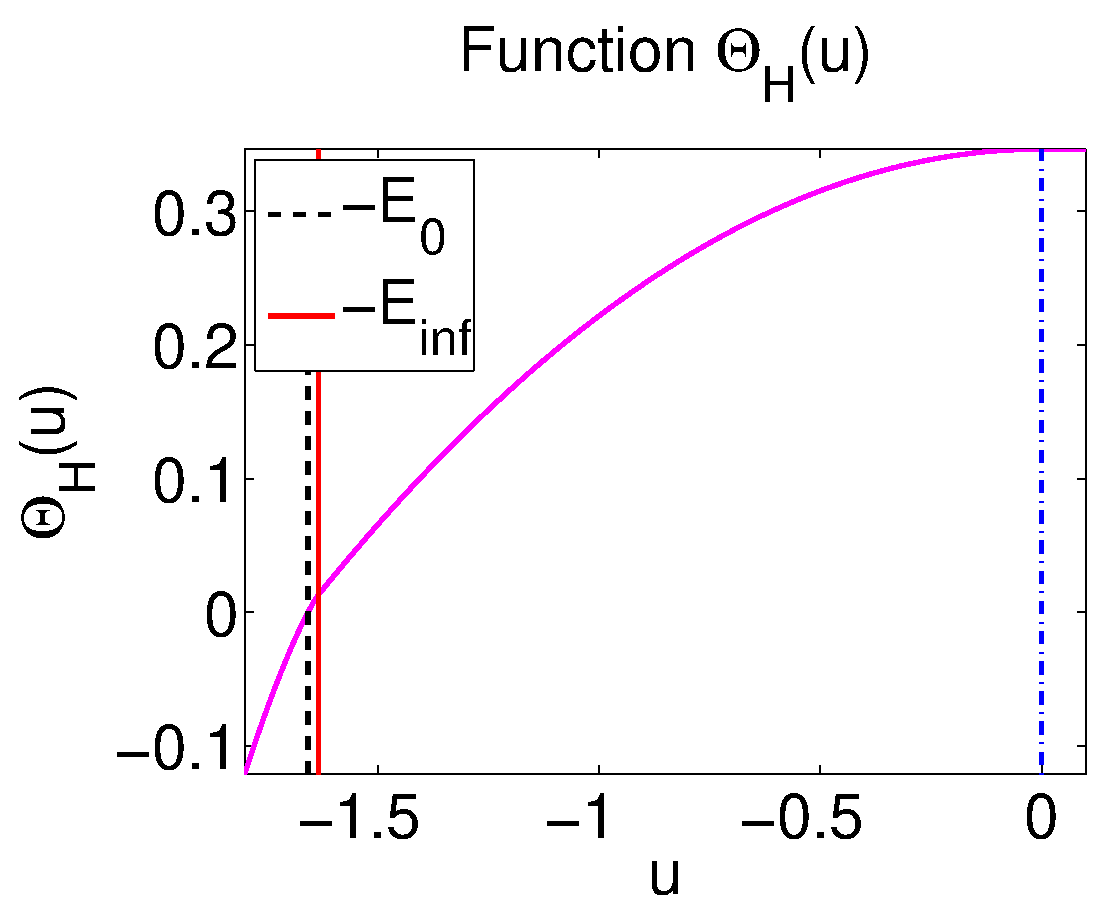
\includegraphics[width = 1.6in]{Theta_cp.pdf}
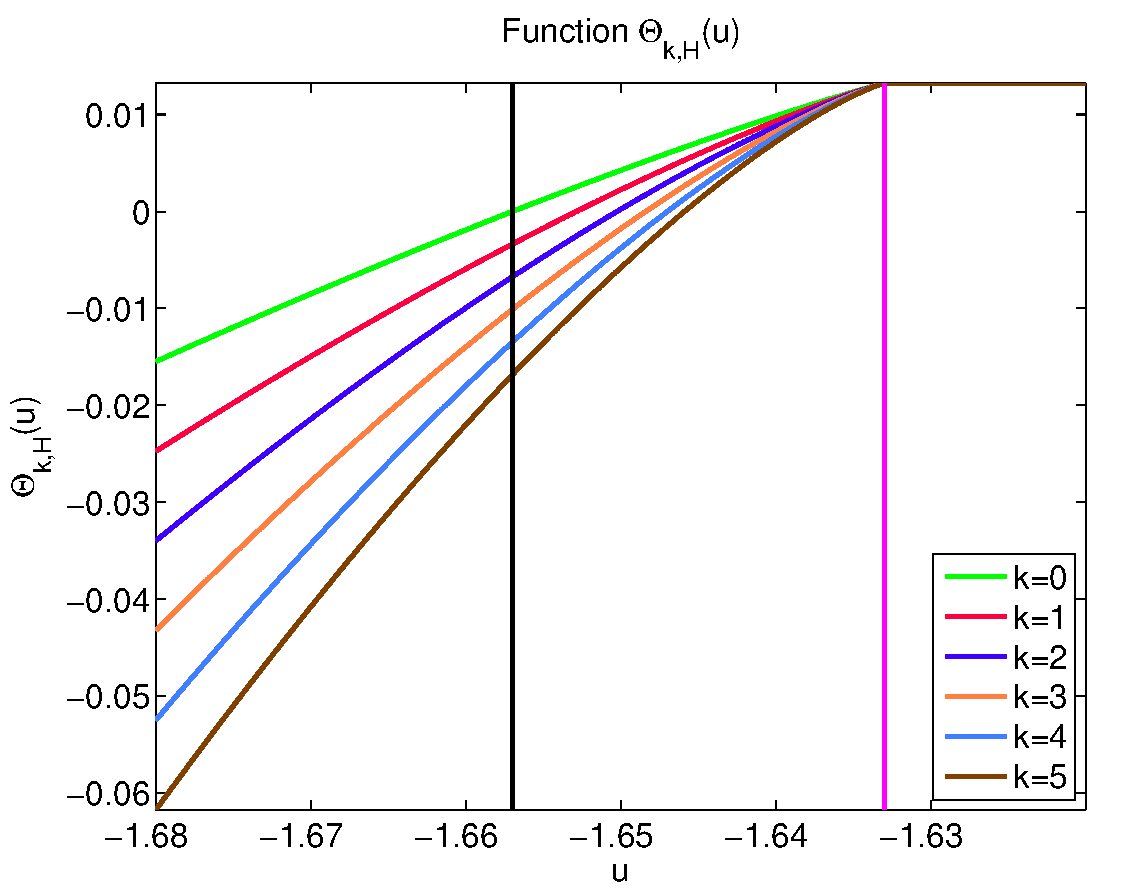
\includegraphics[width = 1.6in]{Theta_lm_sp.pdf}
\vspace{-0.3in}
\caption{Functions $\Theta_H(u)$ and $\Theta_{k,H}(u)$ for $k = \{0,1,\dots,5\}$. Parameter $H$ was set to $H = 3$. Black line: $u = -E_0(H)$, red line: $u = -E_{\infty}(H)$. Notice how narrow band $(-E_0(H),-E_{\infty})$ is. Figure must be read in color.}
\label{fig:Thetas}
%\vspace{-0.05in}
\end{figure}

\begin{corollary}
For all $k > 0$ and $u < -E_{\infty}$, $\Theta_{k,H}(u) < \Theta_{0,H}(u)$.
\label{cor:Theta}
\end{corollary}
Finally, for any integer $k \geq 0$, let $E_k = E_k(H) > 0 $ be defined as the unique solution to 
\[\Theta_{k,H}(-E_k) = 0.
\]

\begin{figure*}[htp!]
  \center
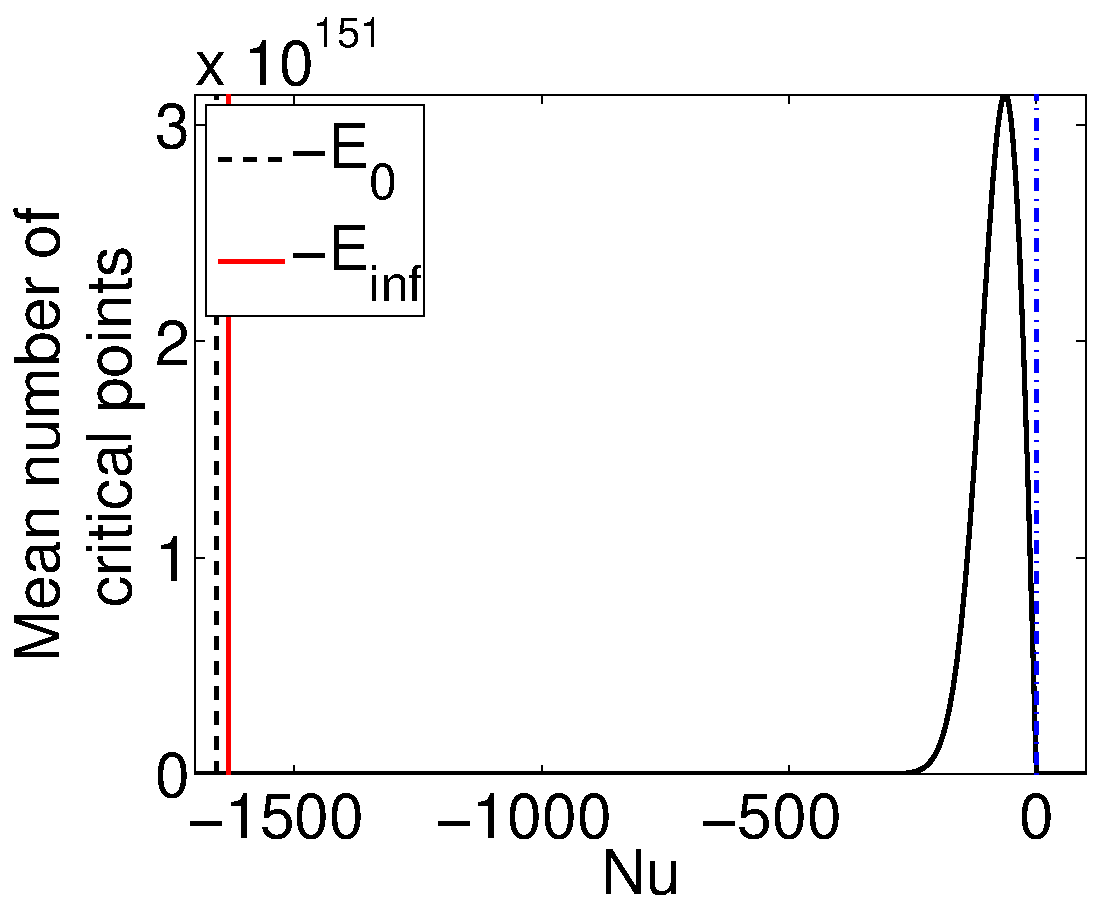
\includegraphics[width = 1.65in]{Distr_cp.pdf}
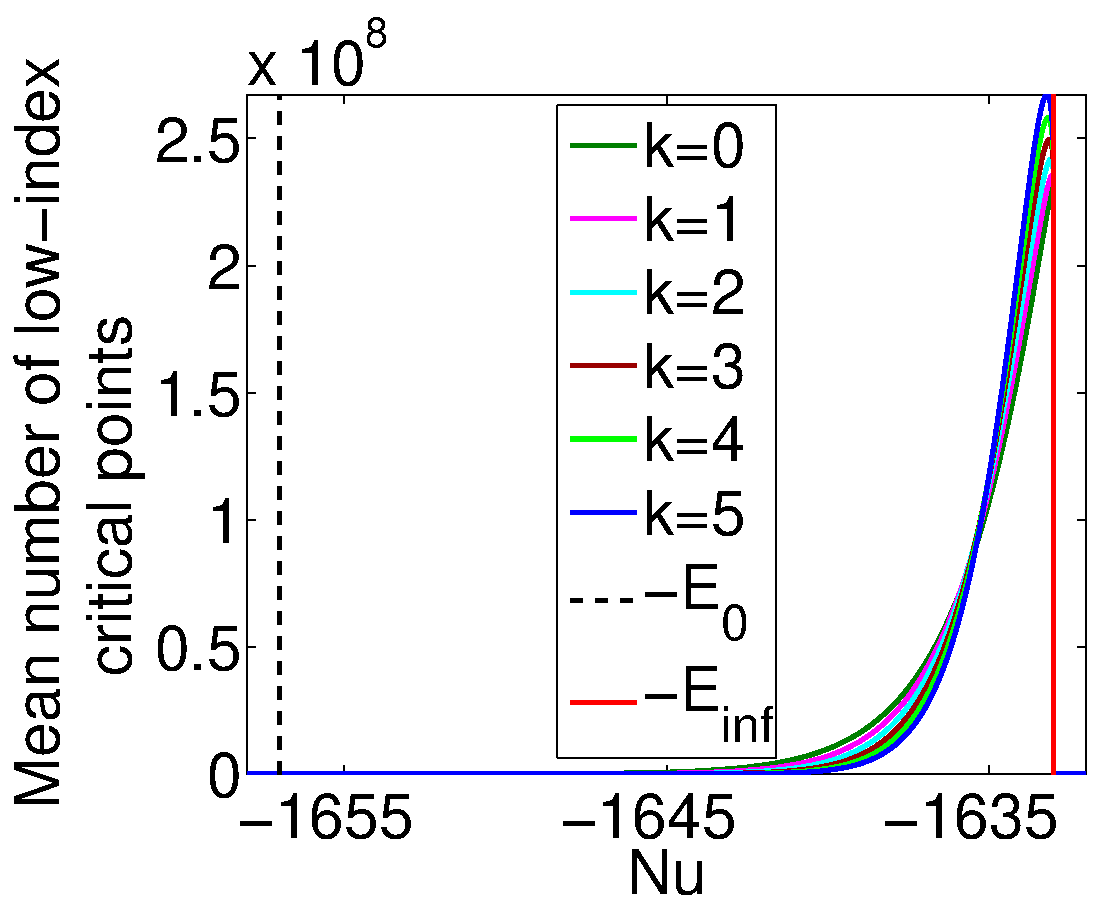
\includegraphics[width = 1.65in]{Distr_lm_sp_li.pdf} 
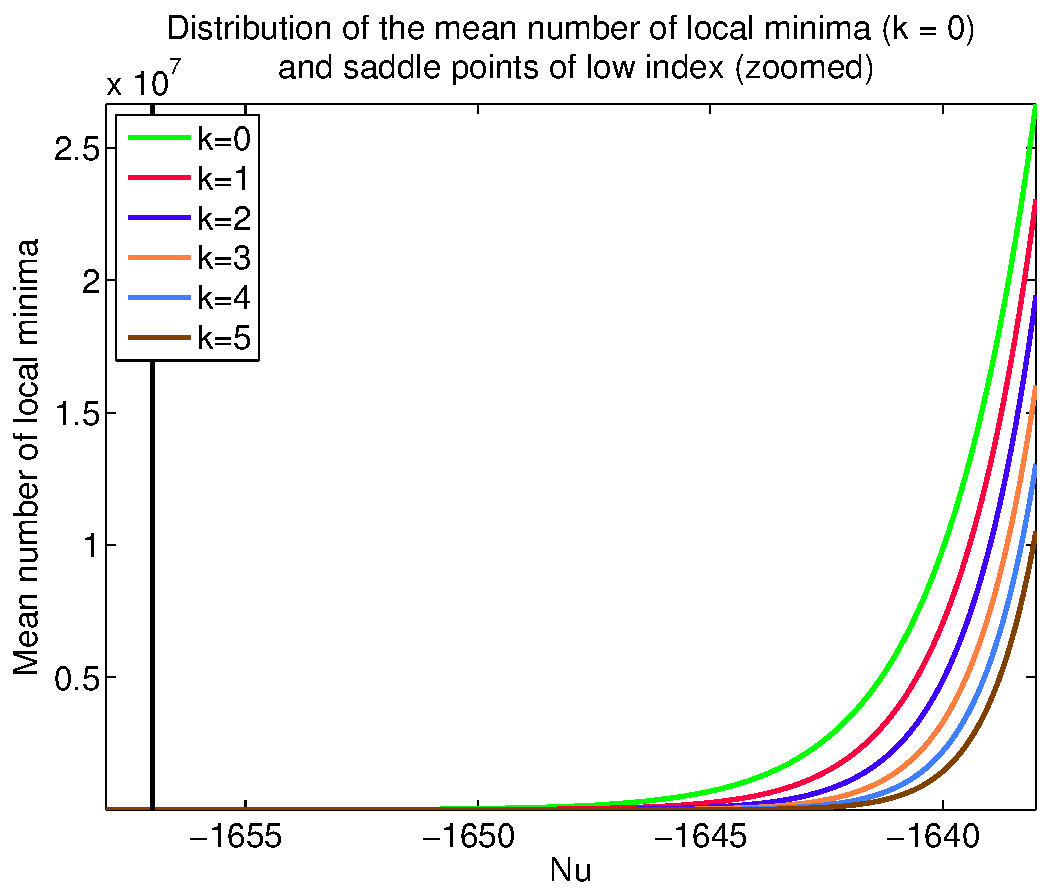
\includegraphics[width = 1.65in]{Distr_lm_sp_li_zoomed_left.pdf} 
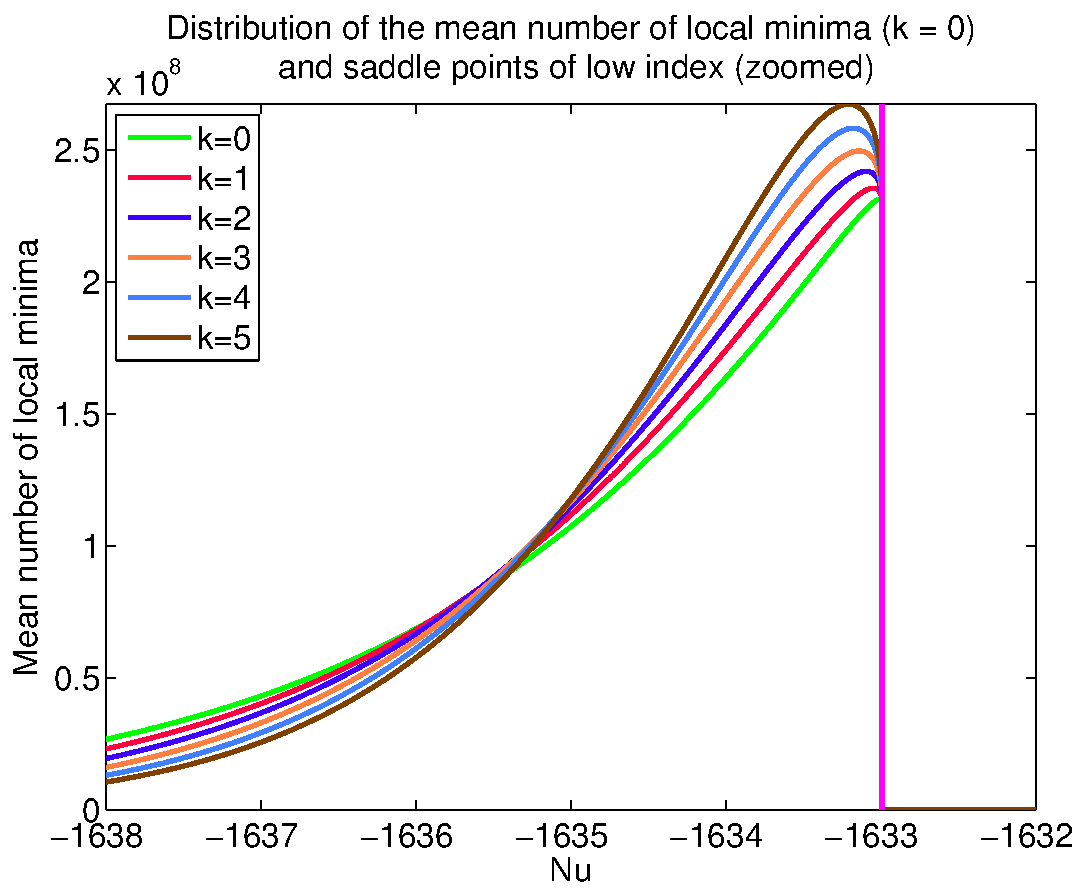
\includegraphics[width = 1.65in]{Distr_lm_sp_li_zoomed_right.pdf} 
\vspace{-0.3in}
\caption{Distribution of the mean number of critical points, local minima and low-index saddle points (oryginal and zoomed). Parameters $H$ and $\Lambda$ were set to $H = 3$ and $\Lambda = 1000$. Black line: $u = -E_0(H)$, red line: $u = -E_{\infty}(H)$. Figure must be read in color.}
\label{fig:Distr_cp_lm_sp}
\vspace{-0.1in}
\end{figure*}

For any fixed $H \geq 3$, the sequence $\{E_k(H)\}_{k\in\mathbb{\Lambda}}$ is strictly decreasing and converges to $E_{\infty}$ as $k \rightarrow \infty$~\cite{AAC2010}. Another important fact is that the band $(-E_0(H),-E_{\infty})$ is very narrow, i.e. it is order of magnitudes narrower than band $(-E_{\infty},0)$. We will now define the ground state energy.

\begin{definition}
The ground state energy is the (normalized) minimum of the loss function $\mathcal{L}_{\Psi,c,H}$
\[G^\Psi = \frac{1}{\Lambda}\inf_{{\bm w}\in \mathcal{S}}\mathcal{L}_{\Lambda,H}({\bm w}).
\]
\end{definition}
Next we provide theorems (resp. Theorem~\ref{thm:lb},~\ref{thm:ub},~\ref{thm:layer}, ~\ref{thm:lmsp} and~\ref{thm:cp}) which are direct consequences of the theoretical findings in~\cite{AAC2010} (resp. Theorem 2.12, 2.14, 2.15, 2.5 and 2.8).  

\begin{theorem}
For every $H \geq 3$
\[\liminf_{\Lambda \rightarrow \infty} G^\Psi \geq -E_0(H),
\]
and for $H \geq 4$
\[\liminf_{\Lambda \rightarrow \infty} G^\Psi = -E_0(H) \:\:\:\text{in probability.}
\]
\label{thm:lb}
\end{theorem}
By Theorem~\ref{thm:lb}, for large-size networks it is improbable to find a critical value below level $-\Lambda E_0(H)$.
\begin{theorem}
For an integer $k \geq 0$ and $\epsilon > 0$,
\[\limsup_{\Lambda \rightarrow \infty} \frac{1}{\Lambda^2}\log(\mathbb{P}(\mathcal{C}_{\Lambda,k}(-E_{\infty}(H) + \epsilon,\infty)>0)) < 0
\]
\label{thm:ub}
\end{theorem}
Theorem~\ref{thm:ub} implies that for large-size networks all critical values of the loss function that are of non-diverging index must lie below the threshold $-\Lambda E_{\infty}(H)$. We will refer to this important threshold as an \textit{energy barrier}. Any critical point that lies above the energy barrier is a high-index saddle point with overwhelming probablity. Theorem~\ref{thm:lb} and~\ref{thm:ub} both imply that for large-size networks all critical values of the loss function that are of non-diverging index must lie in the band $\left(-\Lambda E_0(H),-\Lambda E_{\infty}(H)\right)$.
\begin{theorem}
For $k \geq 0$ and $\epsilon > 0$,
\[\limsup_{\Lambda \rightarrow \infty} \frac{1}{\Lambda^2}\log(\mathbb{P}(\sum_{i=k}^{\infty}\!\mathcal{C}_{\Lambda,i}(-E_k(H) - \epsilon,\infty) \!>\! 0)) \!<\! 0
\]
\label{thm:layer}
\end{theorem}
Theorem~\ref{thm:layer} implies that for large-size networks finding a critical value with index larger or equal to $k$ (for any fixed integer $k$) below energy level $-\Lambda E_k(H)$ is improbable. 

The statements of Theorems~\ref{thm:lb},~\ref{thm:ub} and~\ref{thm:layer} unravel a layered structure for the lowest critical values of the loss function of a large-size network, where with overwhelming probability the critical values above the global minimizer (ground state) of the loss function are local minima exclusively. Above the band ($\left(-\Lambda E_0(H),-\Lambda E_1(H)\right)$) containing only local minima (critical points of index $0$), there is another one, ($\left(-\Lambda E_1(H),-\Lambda E_2(H)\right)$), where one can only find local minima and saddle points of index $1$, and above this band there exists another one, ($\left(-\Lambda E_2(H),-\Lambda E_3(H)\right)$), where one can only find local minima and saddle points of index $1$ and $2$, etc. The above-described layered structure of the lowest critical values of the Hamiltonian of the spherical spin glass model was in-detail described in~\cite{AAC2010}, however with no connection to neural networks which is what we explore. 

An interesting implication of Theorems~\ref{thm:lb},~\ref{thm:ub} and~\ref{thm:layer} is that recovering the global minimizer when starting from any (local) minima from one of the energy bands above, e.g. $\left(-\Lambda E_i(H),-\Lambda E_{i+1}(H)\right)$, diverges with $\Lambda$ since it is bounded below by $\Lambda (E_0(H) - E_i(H))$. 

Next we will show the logarithmic asymptotics of the mean number of critical points (the asymptotics of the mean number of critical points can be found in the Supplementary material).
\begin{theorem}
For all $H \geq 2$ and $k \geq 0$ fixed
\[\lim_{\Lambda \rightarrow \infty}\frac{1}{\Lambda}\log\mathbb{E}[\mathcal{C}_{\Lambda,k}(u)] = \Theta_{k,H}(u).
\]
\label{thm:lmsp}
\end{theorem}
\begin{theorem}
For all $H \geq 2$
\[\lim_{\Lambda \rightarrow \infty}\frac{1}{\Lambda}\log\mathbb{E}[\mathcal{C}_{\Lambda}(u)] = \Theta_{H}(u).
\]
\label{thm:cp}
\end{theorem}
Note that from Theorem~\ref{thm:lmsp} and Corollary~\ref{cor:Theta} it follows that the number of critical points in the band $\left(-\Lambda E_0(H),-\Lambda E_{\infty}(H)\right)$ increases exponentially as $\Lambda$ grows and that local minima dominate over saddle points and this domination also grows exponentially as $\Lambda$ grows. Thus for large-size networks (large $\Lambda$) the probability of recovering a saddle point in the band $\left(-\Lambda E_0(H),-\Lambda E_{\infty}(H)\right)$, rather than a local minima, goes to $0$.

Figure~\ref{fig:Distr_cp_lm_sp} captures exemplary plots of the distributions of the mean number of critical points, local minima and low-index saddle points. Clearly local minima and low-index saddle points are located in the band $\left(-\Lambda E_0(H),-\Lambda E_{\infty}(H)\right)$ whereas high-index saddle points can only be found above the energy barrier $-\Lambda E_{\infty}(H)$. Figure~\ref{fig:Distr_cp_lm_sp} also reveals the layered structure for the lowest critical values of the loss function. 

\section{Experiments}
\label{sec:Experiments}

\textcolor{red}{We need to prove that we get ot local minima not flat saddle points from Bengio paper.}

\section{Conclusion and Future Work}
\label{sec:ConandFutWork}

\bibliographystyle{apalike}
\bibliography{PAPER_AMMLY}

\clearpage

\toptitlebar 
{\Large \bf  \centering{Deep-optimization with large networks\\(Supplementary Material)} \par}
\bottomtitlebar

\section{Proof of Theorem~\ref{thm:arge}}
\begin{proof}
First we will prove the lower-bound. By the inequality between arithmetic and geometric mean the mass and the size of the network are connected as follows
\[\Lambda \geq \sqrt[H]{\Psi^2}\frac{H}{\sqrt[H]{n_0n_H}} = \sqrt[H]{\Psi^2}\frac{H}{\sqrt[H]{d}},
\]
and since $\sqrt[H]{\Psi}\frac{H}{\sqrt[H]{d}} = \sqrt[H]{\prod_{i = 1}^{H}n_i}H \geq 1$ then 
\[\Lambda \geq \sqrt[H]{\Psi^2}\frac{H}{\sqrt[H]{d}} \geq \sqrt[H]{\Psi}.
\]
The upper-bound can be shown as follows
\[\Lambda \leq \prod_{i=0}^{H-1}n_in_{i+1} = \frac{\Psi^2}{n_0n_H} = \Psi^2\frac{1}{d}.
\]
\end{proof}

\section{Proof of Theorem~\ref{thm:redun}}
\begin{proof}
We will first proof the following more general lemma.
\begin{lemma}
Let $Y_1$ and $Y_2$ be the outputs of two arbitrary binary classifiers. Assume that the first classifiers predicts $1$ with probability $p$ where, without loss of generality, we assume $p \leq 0.5$ and $-1$ otherwise. Furthemore, let the prediction accuracy of the second classifier differ from the prediction accuracy of the first classifier by no more than $\epsilon \in [0,p]$. Then the following holds
\[corr(sign(Y_1),sign(Y_2)) \geq \frac{2p(1 \!-\! p \!+\! \epsilon) \!-\! \epsilon}{2\sqrt{(p \!+\! \epsilon)(1 \!-\! p \!+\! \epsilon)p(1 \!-\! p)}}.
\]
\end{lemma}
\begin{proof}
Consider two random variables $Z_1 = sign(Y_1)$ and $Z_2 = sign(Y_2)$. Let $\mathcal{X}^{+}$ denote the set of data points for which the first classifier predicts $+1$ and let $\mathcal{X}^{-}$ denote the set of data points for which the first classifier predicts $-1$ ($\mathcal{X}^{+} \cup \mathcal{X}^{-} = \mathcal{X}$, where $\mathcal{X}$ is the entire dataset). Also let $p = \frac{|\mathcal{X}^{+}|}{|\mathcal{X}|}$. Furthermore, let $\mathcal{X}_{\epsilon}^{-}$ denote the dataset for which $Z_1 = +1$ and $Z_2 = -1$ and $\mathcal{X}_{\epsilon}^{+}$ denote the dataset for which $Z_1 = -1$ and $Z_2 = +1$, where $\frac{|\mathcal{X}_{\epsilon}^{+}| + |\mathcal{X}_{\epsilon}^{-}|}{\mathcal{X}} = \epsilon$. Also let $\epsilon^{+} = \frac{|\mathcal{X}_{\epsilon}^{+}|}{\mathcal{X}}$ and $\epsilon^{-} = \frac{|\mathcal{X}_{\epsilon}^{-}|}{\mathcal{X}}$. Therefore
\[Z_1 \!=\! \left \{
  \begin{tabular}{c}
  $1$ \:\:if $x \in \mathcal{X}^{+}$\\
  \!\!\!\!$-1$ \:\:if $x \in \mathcal{X}^{-}$
  \end{tabular}
\right.
\]
and
\[Z_2 \!=\! \left \{
  \begin{tabular}{c}
  $1$ \:\:if $x \in \mathcal{X}^{+} \cup \mathcal{X}_{\epsilon}^{+}  \setminus \mathcal{X}_{\epsilon}^{-}$\\
  \!\!\!$-1$ \:\:if $x \in \mathcal{X}^{-} \cup \mathcal{X}_{\epsilon}^{-} \setminus \mathcal{X}_{\epsilon}^{+}$.
  \end{tabular}
\right.
\]
One can compute that $\mathbb{E}[Z_1] = 2p-1$, $\mathbb{E}[Z_2] = 2(p + \epsilon^{+} - \epsilon^{-}) - 1$, $\mathbb{E}[Z_1Z_2] = 1 - 2\epsilon$, $std(Z_s) = 2\sqrt{p(1-p)}$, and finally $std(Z_\Lambda) = 2\sqrt{(p + \epsilon^{+} - \epsilon^{-})(1 - p - \epsilon^{+} + \epsilon^{-})}$.
Thus we obtain
\begin{eqnarray}
&&\!\!\!\!\!\!\!\!\!\!\!\!\!\!\!corr(sign(Y_1),sign(Y_2)) = corr(Z_1,Z_2) \nonumber\\
&\!\!\!\!\!\!\!\!\!\!\!\!\!\!\!=& \!\!\!\!\!\!\!\!\!\!\frac{\mathbb{E}[Z_1Z_2] - \mathbb{E}[Z_1]\mathbb{E}[Z_2]}{std(Z_1)std(Z_2)} \nonumber\\
&\!\!\!\!\!\!\!\!\!\!\!\!\!\!\!=& \!\!\!\!\!\!\!\!\!\!\frac{1 - 2\epsilon - (1 - 2p)^2 + 2(1 - 2p)(\epsilon^{+} - \epsilon^{-})}{4\sqrt{p(1 - p)(p + \epsilon^{+} - \epsilon^{-})(1 - p - \epsilon^{+} + \epsilon^{-})}} \nonumber\\
&\!\!\!\!\!\!\!\!\!\!\!\!\!\!\!\geq& \!\!\!\!\!\!\!\!\!\!\frac{1 - 2\epsilon - (1 - 2p)^2 - 2(1 - 2p)\epsilon}{4\sqrt{p(1 - p)(p + \epsilon)(1 - p + \epsilon)}}
\label{eq:tmp}
\end{eqnarray}
\end{proof}
Note that when the first classifier is network $\mathcal{N}$ considered in this paper and $\mathcal{M}$ is its $(s,\epsilon)$-reduction image $\mathbb{E}[Y_1] = 0$ and $\mathbb{E}[Y_2] = 0$ (that follows from the fact that $X$'s in Equation~\ref{eq:befapprox} have zero-mean). That implies $p=0.5$ which, when substituted to Equation~\ref{eq:tmp} gives the theorem statement.
\end{proof}

\section{Proof of Lemma~\ref{lem:tmp2}}

The decomposability of $X_{i_1,\dots,i_H}^{(j)}$ implies that for independend standard normal random variables $Z$'s the following holds:
\begin{eqnarray*}
\sum_{j=1}^{r_{i_1,\dots,i_H}^{'}}X_{i_1,\dots,i_H}^{(j)} &\!\!\!\!\!=& \!\!\!\!\!\sum_{j=1}^{r_{i_1,\dots,i_H}^{'}}\hat{r}_{i_1,\dots,i_H}\sum_{k=1}^{\frac{1}{\hat{r}_{i_1,\dots,i_H}^2}}Z_{i_1,\dots,i_H}^{(j,k)}\\
&\!\!\!\!\!=& \!\!\!\!\!\sum_{j=1}^{r_{i_1,\dots,i_H}^{''}}\hat{r}_{i_1,\dots,i_H}Z_{i_1,\dots,i_H}^{(j)},
\end{eqnarray*}
where the last step comes from combining both summations and re-indexing the summands. Therefore
\begin{eqnarray*}
Y_s &=& q\sum_{i_1,\dots,i_H=1}^{s}\sum_{j=1}^{r_{i_1,\dots,i_H}^{''}}\hat{r}_{i_1,\dots,i_H}Z_{i_1,\dots,i_H}^{(j)}\rho\prod_{k = 1}^{H}w_{i_k}\\
&=& \sum_{i_1,\dots,i_H=1}^{\Lambda}\hat{r}_{i_1,\dots,i_H}Z_{i_1,\dots,i_H}\rho\prod_{k = 1}^{H}w_{i_k},
\end{eqnarray*}
where the last step comes again from combining both summations and re-indexing the summands. 

\section{Proof of Theorem~\ref{thm:unif}}
\begin{proof}
Note that $\mathbb{E}[\hat{Y}_s] = 0$ and $\mathbb{E}[Y_{\Lambda}] = 0$. Furthermore
\[\mathbb{E}[\hat{Y}_sY_{\Lambda}] = q^2\rho^2\sum_{i_1,i_2,\dots,i_H=1}^{\Lambda}\sqrt{\frac{\Psi}{\Lambda^H}}\hat{r}_{i_1,i_2,\dots,i_H}\prod_{k = 1}^{H}w_{i_k}^2
\]
and
\[std(\hat{Y}_s) = q\rho\sqrt{\sum_{i_1,i_2,\dots,i_H=1}^{\Lambda}\frac{\Psi}{\Lambda^H}\prod_{k = 1}^{H}w_{i_k}^2}
\]
\[std(Y_{\Lambda}) = q\rho\sqrt{\sum_{i_1,i_2,\dots,i_H=1}^{\Lambda}\hat{r}_{i_1,i_2,\dots,i_H}^2\prod_{k = 1}^{H}w_{i_k}^2}.
\]
Therefore
\begin{eqnarray*}
&&\!\!\!\!\!\!\!\!\!corr(\hat{Y}_s,Y_{\Lambda})\\ 
&\!\!\!\!\!\!\!\!\!=&\!\!\!\!\!\!\! \frac{\displaystyle\sum_{i_1,\dots,i_H=1}^{\Lambda}\sqrt{\frac{\Psi}{\Lambda^H}}\hat{r}_{i_1,\dots,i_H}\prod_{k = 1}^{H}w_{i_k}^2}{\sqrt{\!\!\!\left(\displaystyle\sum_{i_1,\dots,i_H=1}^{\Lambda}\frac{\Psi}{\Lambda^H}\prod_{k = 1}^{H}w_{i_k}^2\right)\!\!\!\!\left(\displaystyle\sum_{i_1,\dots,i_H=1}^{\Lambda}\!\!\!\!\!\hat{r}_{i_1,\dots,i_H}^2\prod_{k = 1}^{H}w_{i_k}^2\right)}}\\
&\!\!\!\!\!\!\!\!\geq& \delta, 
\end{eqnarray*}
where the last inequality is the direct consequence of the uniformity assumption of Equation~\ref{eq:uniform}.
\end{proof}

\begin{comment}
\section{Approximation of 2-spin Spin Glasses by 1-layer Neural Networks}

The Hamiltonian of a H-spin glass is given by 

\begin{equation}
 S_H(w) = \sum_{i_1,...,i_H}^N x_{i_1,...,i_H} w_{i_1} \cdot ... \cdot w_{i_H}
\end{equation}
and the output of a deep linear network with $H$ layers by 
\begin{equation}
 Y_H(w) = \sum_{p = (i_1,...,i_H) \in \mathcal{P}} x_{i_1,...,i_H} w_{i_1} \cdot ... \cdot w_{i_H}
\end{equation}

Here $\mathcal{P}$ denotes the set of all paths from inputs to outputs in the network. Let $\mathcal{U} = \{ w_{i_1} \cdot ... \cdot w_{i_H} : 1 \leq i_1,...,i_H \leq N \} $.
Note that the number of terms in the sum $S_H(w)$ is equal to $|\mathcal{U}| = N^H$ and the number of terms in $Y_H(w)$ is equal to $|\mathcal{P}|$.

\begin{definition}
 Let $P_1(w), P_2(w)$ be random polynomials in $w$, where $w \in \mathbb{R}^N$, and let $m_1,m_2$ be the number of nonzero terms in $P_1,P_2$. Assume that all nonzero terms which appear in $P_1$ also appear in $P_2$. 
 We define a measure of similarity between the polynomials as $\Phi(P_1,P_2) = \frac{m_1}{m_2}$.
\end{definition}

\begin{lemma}
Consider the following network $\mathcal{N}$ whose output is given by $Y(w) = \sum \sigma Wx$, where $\sigma$ is a rectified linear unit non-linearity.
Furthermore assume that $rank(W) = k$.
Then $\Phi(Y(w),S(w))  = \frac{1}{4k}$.
\end{lemma}

\begin{proof}
 Assume for simplicity that $W$ is $n \times n$. Since $W$ has rank $k$, it can be written as $W = UV^T$, where $U$ and $V$ have dimension $n \times k$.
 We can therefore reparameterize the system so that the free parameters consist of the entries of $U$ and $V$, which brings the number of parameters to $2kn$. 
 Assume these are reindexed of the form $\{w_1,w_2,...,w_{2kn} \}$.
 A spin glass model with this set of parameters and $H=2$ will have $(2kn)^2=4k^2n^2$ terms in its sum.
 Let us now count the number of unique terms in the polynomial $Y(w)$ which represents our network. 
 The matrix $W = UV^T$ has $n^2$ entries, each of which is of the form $u^Tv$ for some row $u$ of $U$ and $v$ of $V$. 
 Since $u,v \in \mathbb{R}^k$, each entry is the sum of $k$ terms of the form $w_i w_j$. 
 It follows that each entry in the column vector $Wx$ is the sum of $nk$ terms, and hence the output $y$ is the sum of $n^2k$ terms, all of the form $w_iw_jx_{ij}$.
 We thus have $\Phi(Y(w),S(w)) = \frac{n^2k}{4n^2k^2} = \frac{1}{4k}$.
\end{proof}

  In the above example, we can combine pairs of terms of the form $w_iw_jx_{ij} + w_jw_ix_{ji}$ into $w_iw_j(x_{ij}+x_{ji})$. 
  The sum $(x_{ij}+x_{ji})$ has higher variance than the other input terms, but if this is a benign assumption for subsequent results then the ratio of terms becomes $\frac{1}{2k}$ rather than $\frac{1}{4k}$.

\begin{lemma}
 The class of functions which can be learned by networks of the form $y = v^T \sigma Wx$ and $y = \sum \sigma Wx$ is equivalent. 
\end{lemma}

\begin{proof}
 We can show this by simple change of variables. 
 \begin{align*}
  y &= v^T \sigma(Wx) \\
  &= \sum_i v_i \sigma(\sum_j w_{ij} x_j) \\
  &= \sum_i \sigma(\sum_j v_i w_{ij} x_j) \\
  &= \sum_i \sigma(\sum_j w_{ij}' x_j) \\
  &= \sum_i \sigma(W'x)
 \end{align*}
 
 where $w_{ij}' = v_i w_{ij}$.
\end{proof}

\begin{theorem}
 Let $Y(w)$ be the output of a one-layer linear network, $S(w)$ be the Hamiltonian of a 2-spin spin glass model, and assume that the weights of $Y$ have rank $k$. 
 Then $\Phi(Y(w),S(w)) = \frac{1}{4k}$.
\end{theorem}

\begin{proof}
 This follows directly from the two above lemmas.
\end{proof}
\end{comment}

\section{Asymptotics of the mean number of critical points and local minima}

Below, we provide the asymptotics of the mean number of critical points (Theorem~\ref{thm:cpprecise}) and the mean number of local minima (Theorem~\ref{thm:lmspprecise}), which extend Theorem~\ref{thm:lmsp} and Theorem~\ref{thm:cp}. Those results are the consequences of Theorem 2.17. and Corollary 2.18.~\cite{AAC2010} and the boundeness of $c$ and $H$.
\begin{theorem}
For $H \geq 3$, the following holds as $\Lambda \rightarrow \infty$:
\begin{itemize}
\item For $u < -E_{\infty}$\\
\begin{eqnarray*}
\mathbb{E}[\mathcal{C}_{\Lambda}(u)] \!\!\!&=&\!\!\! \frac{h(v)}{\sqrt{2H\pi}}\frac{\exp(I_1(v) - \frac{v}{2}I_1^{'}(v))}{-\Phi^{'}(v) + I_1^{'}(v)}\Lambda^{-\frac{1}{2}}\\
&\cdot& \exp\left(\Lambda\Theta_H(u)\right)(1 + o(1)),
\end{eqnarray*}
where $v = -u\sqrt{\frac{H}{2(H-1)}}$, $\Phi(v) = -\frac{H-2}{2H}v^2$,\\
$h(v) = \left|\frac{v-\sqrt{2}}{v + \sqrt{2}}\right|^{\frac{1}{4}} + \left|\frac{v+\sqrt{2}}{v - \sqrt{2}}\right|^{\frac{1}{4}}$\\
and $I_1(v) = \int_{\sqrt{2}}^{v}\sqrt{|x^2 - 2|}dx$.
\item For $u = -E_{\infty}$\\
\begin{eqnarray*}
\mathbb{E}[\mathcal{C}_{\Lambda}(u)] = \frac{2A(0)\sqrt{2H}}{3(H-2)}\Lambda^{-\frac{1}{3}}\\
\cdot\exp\left(\Lambda\Theta_H(u)\right)(1 + o(1)),
\end{eqnarray*}
where $A$ is the Airy function of first kind.
\item For $u \in (-E_{\infty},0)$\\
\begin{eqnarray*}
\mathbb{E}[\mathcal{C}_{\Lambda}(u)] = \frac{2\sqrt{2H(E_{\infty}^2-u^2)}}{(2-H)\pi u}\\
\cdot\exp\left(\Lambda \Theta_H(u)\right)(1 + o(1)),
\end{eqnarray*}
\item For $u > 0$\\
\begin{eqnarray*}
\mathbb{E}[\mathcal{C}_{\Lambda}(u)] = \frac{4\sqrt{2}}{\sqrt{\pi(H-2)}}\Lambda^{\frac{1}{2}}\\
\cdot\exp\left(\Lambda\Theta_H(0)\right)(1 + o(1)),
\end{eqnarray*}
\end{itemize}
\label{thm:cpprecise}
\end{theorem}
\begin{theorem}
For $H \geq 3$ and $u < -E_{\infty}$, the following holds as $\Lambda \rightarrow \infty$:
\begin{eqnarray*}
\mathbb{E}[\mathcal{C}_{\Lambda,0}(u)] \!\!\!&=&\!\!\! \frac{h(v)}{\sqrt{2H\pi}}\frac{\exp(I_1(v) - \frac{v}{2}I_1^{'}(v))}{-\Phi^{'}(v) + I_1^{'}(v)}\Lambda^{-\frac{1}{2}}\\
&\cdot& \exp\left(\Lambda\Theta_H(u)\right)(1 + o(1)),
\end{eqnarray*}
where $v$, $\Phi$, $h$ and $I_1$ were defined in Theorem~\ref{thm:cpprecise}.
\label{thm:lmspprecise}
\end{theorem}

\end{document}
